\chapter{不定积分}

\section{不定积分概念与基本积分公式}

正如加法有其逆运算减法, 乘法有其逆运算除法一样, 微分法也有它的逆运算——积分法. 我们已经知道, 微分法的基本问题是研究如何从已知函数求出它的导函数,那么与之相反的问题是:求一个未知函数,使其导函数恰好是某一已知函数. 提出这个逆问题,首先是因为它出现在许多实际问题之中. 例如:已知速度求路程； 已知加速度求速度; 已知曲线上每一点处的切线斜率 (或斜率所满足的某一规律), 求曲线方程; 等等. 本章与其后两章 (定积分与定积分的应用) 构成一元函数积分学.

\subsection{原函数与不定积分}

%定义  1
\begin{definition}{}{def:}

\end{definition}
设函数 \(f\) 与 \(F\) 在区间 \(I\) 上都有定义. 若
\[
{F}^{\prime }\left( x\right)  = f\left( x\right) ,\;x \in  I,
\]
则称 \(F\) 为 \(f\) 在区间 \(I\) 上的一个原函数.

例如, \(\frac{1}{3}{x}^{3}\) 是 \({x}^{2}\) 在 \(\left( {-\infty , + \infty }\right)\) 上的一个原函数,因为 \({\left( \frac{1}{3}{x}^{3}\right) }^{\prime } = {x}^{2}\) ;

又如 \(- \frac{1}{2}\cos {2x}\) 与 \(- \frac{1}{2}\cos {2x} + 1\) 都是 \(\sin {2x}\) 在 \(\left( {-\infty , + \infty }\right)\) 上的原函数,因为
\[
{\left( -\frac{1}{2}\cos 2x\right) }^{\prime } = {\left( -\frac{1}{2}\cos 2x + 1\right) }^{\prime } = \sin {2x}.
\]
如果这些简单的例子都可从基本求导公式反推而得的话, 那么
\[
F\left( x\right)  = x\arctan x - \frac{1}{2}\ln \left( {1 + {x}^{2}}\right)
\]
是 \(f\left( x\right)  = \arctan x\) 的一个原函数,就不那样明显了. 事实上,研究原函数必须解决下面两个重要问题:

1. 满足何种条件的函数必定存在原函数? 如果存在, 是否唯一?

2. 若已知某个函数的原函数存在, 又怎样把它求出来?

关于第一个问题,我们用下面两个定理来回答；至于第二个问题,其解答则是本章接着要介绍的各种积分方法.

%定理 8.1
\begin{theorem}{}{the:}

\end{theorem}
 若函数 \(f\) 在区间 \(I\) 上连续,则 \(f\) 在 \(I\) 上存在原函数 \(F\) ,即 \({F}^{\prime }\left( x\right)  =\)  \(f\left( x\right) ,x \in  I\) .

本定理要到第九章 §5 中才能获得证明.

由于初等函数在其定义区间上为连续函数, 因此每个初等函数在其定义区间上都有原函数 (只是初等函数的原函数不一定仍是初等函数). 当然, 一个函数如果存在间断点, 那么此函数在其间断点所在的区间上就不一定存在原函数 (参见本节习题第 4 题和第 8 题).

%定理 8.2
\begin{theorem}{}{the:}

\end{theorem}
 设 \(F\) 是 \(f\) 在区间 \(I\) 上的一个原函数,则

(i) \(F + C\) 也是 \(f\) 在 \(I\) 上的原函数,其中 \(C\) 为任意常量函数\footnote{这里既把 \(C\) 看作常量函数,又把它作为该常量函数的函数值. 在不致混淆时,以后常说 “ \(C\) 为任意常数”.};

(ii) \(f\) 在 \(I\) 上的任意两个原函数之间,只可能相差一个常数.

%证
\begin{proof}

\end{proof}
(i) 这是因为 \({\left\lbrack  F\left( x\right)  + C\right\rbrack  }^{\prime } = {F}^{\prime }\left( x\right)  = f\left( x\right) ,x \in  I\) .

(ii) 设 \(F\) 和 \(G\) 是 \(f\) 在 \(I\) 上的任意两个原函数,则有
\[
{\left\lbrack  F\left( x\right)  - G\left( x\right) \right\rbrack  }^{\prime } = {F}^{\prime }\left( x\right)  - {G}^{\prime }\left( x\right)
\]
\[
= f\left( x\right)  - f\left( x\right)  = 0,\;x \in  I.
\]
根据第六章拉格朗日中值定理的推论, 知道
\[
F\left( x\right)  - G\left( x\right)  \equiv  C,\;x \in  I.
\]
%定义  2
\begin{definition}{}{def:}

\end{definition}
函数 \(f\) 在区间 \(I\) 上的全体原函数称为 \(f\) 在 \(I\) 上的不定积分,记作
\[
\int f\left( x\right) \mathrm{d}x, \tag{1}
\]
其中称 \(\int\) 为积分号, \(f\left( x\right)\) 为被积函数, \(f\left( x\right) \mathrm{d}x\) 为被积表达式 \footnote{不久可看到,被积表达式可认同为 \(f\) 的原函数 \(F\) 的微分,即 \(\mathrm{d}F = {F}^{\prime }\left( x\right) \mathrm{d}x = f\left( x\right) \mathrm{d}x\) .} , \(x\) 为积分变量. 尽管记号 (1)中各个部分都有其特定的名称,但在使用时必须把它们看作一个整体.

由定义 2 可见,不定积分与原函数是总体与个体的关系,即若 \(F\) 是 \(f\) 的一个原函数,则 \(f\) 的不定积分是一个函数族 \(\{ F + C\}\) ,其中 \(C\) 是任意常数. 为方便起见,写作
\[
\int f\left( x\right) \mathrm{d}x = F\left( x\right)  + C. \tag{2}
\]
这时又称 \(C\) 为积分常数,它可取任一实数值. 于是又有
\[
{\left\lbrack  \int f\left( x\right) \mathrm{d}x\right\rbrack  }^{\prime } = {\left\lbrack  F\left( x\right)  + C\right\rbrack  }^{\prime } = f\left( x\right) , \tag{3}
\]
\[
\mathrm{d}\int f\left( x\right) \mathrm{d}x = \mathrm{d}\left\lbrack  {F\left( x\right)  + C}\right\rbrack   = f\left( x\right) \mathrm{d}x. \tag{4}
\]
按照写法 (2), 本节开头所举的几个例子可写作
\[
\int {x}^{2}\mathrm{\;d}x = \frac{1}{3}{x}^{3} + C,
\]
\[
\int \sin {2x}\mathrm{\;d}x =  - \frac{1}{2}\cos {2x} + C,
\]
\[
\int \arctan x\mathrm{\;d}x = x\arctan x - \frac{1}{2}\ln \left( {1 + {x}^{2}}\right)  + C.
\]
此外, 一个函数 “存在不定积分” 与 “存在原函数” 显然是等同的说法.

不定积分的几何意义 若 \(F\) 是 \(f\) 的一个原函数,则称 \(y = F\left( x\right)\) 的图像为 \(f\) 的一条积分曲线. 于是, \(f\) 的不定积分在几何上表示 \(f\) 的某一积分曲线沿纵轴方向任意平移所得一切积分曲线组成的曲线族 (图 8-1). 显然, 若在每一条积分曲线上横坐标相同的点处作切线, 则这些切线互相平行.

\begin{figure}
	\centering
	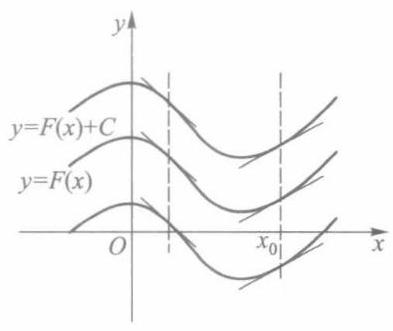
\includegraphics[width=.3\textwidth]{images/P050.jpg}
	\caption{图 $8-1$}
	\label{fig:P050}
\end{figure}

在求原函数的具体问题中, 往往先求出全体原函数,然后从中确定一个满足条件 \(F\left( {x}_{0}\right)  = {y}_{0}\) (称为初始条件,它由具体问题所规定) 的原函数,它就是积分曲线族中通过点 \(\left( {{x}_{0},{y}_{0}}\right)\) 的那一条积分曲线. 例如,质点做匀加速直线运动时, \(a\left( t\right)  = {v}^{\prime }\left( t\right)  = a\) ,则
\[
v\left( t\right)  = \int a\mathrm{\;d}t = {at} + C.
\]
若已知 \(v\left( {t}_{0}\right)  = {v}_{0}\) ,代入上式后确定积分常数 \(C = {v}_{0} - a{t}_{0}\) ,于是就有
\[
v\left( t\right)  = a\left( {t - {t}_{0}}\right)  + {v}_{0}.
\]
又因 \({s}^{\prime }\left( t\right)  = v\left( t\right)\) ,所以又有
\[
s\left( t\right)  = \int \left\lbrack  {a\left( {t - {t}_{0}}\right)  + {v}_{0}}\right\rbrack  \mathrm{d}t = \frac{1}{2}a{\left( t - {t}_{0}\right) }^{2} + {v}_{0}t + {C}_{1}.
\]
若已知 \(s\left( {t}_{0}\right)  = {s}_{0}\) ,则 \({C}_{1} = {s}_{0} - {v}_{0}{t}_{0}\) ,代入上式得到
\[
s\left( t\right)  = \frac{1}{2}a{\left( t - {t}_{0}\right) }^{2} + {v}_{0}\left( {t - {t}_{0}}\right)  + {s}_{0}.
\]
\subsection{基本积分表}

怎样求原函数? 读者很快就会发现这要比求导数困难得多. 原因在于原函数的定义不像导数定义那样具有构造性,即它只告诉我们其导数恰好等于某个已知函数 \(f\) ,而没有指出怎样由 \(f\) 求出它的原函数的具体形式和途径. 因此,我们只能先按照微分法的已知结果去试探.

首先, 我们把基本导数公式改写成基本积分公式:

1. \(\int 0\mathrm{\;d}x = C\) .

2. \(\int 1\mathrm{\;d}x = \int \mathrm{d}x = x + C\) .

3. \(\int {x}^{\alpha }\mathrm{d}x = \frac{{x}^{\alpha  + 1}}{\alpha  + 1} + C\left( {\alpha  \neq   - 1,x > 0}\right)\) .

4. \(\int \frac{1}{x}\mathrm{\;d}x = \ln \left| x\right|  + {C}\footnote{公式 4 适用于不含坐标原点的任何区间,读者容易验证\[
{\left( \ln \left| x\right|  + C\right) }^{\prime } = \frac{1}{x},x \neq  0.
\]
}\left( {x \neq  0}\right)\) .



5. \(\int {\mathrm{e}}^{x}\mathrm{\;d}x = {\mathrm{e}}^{x} + C\) .

6. \(\int {a}^{x}\mathrm{\;d}x = \frac{{a}^{x}}{\ln a} + C\left( {a > 0,a \neq  1}\right)\) .

7. \(\int \cos {ax}\mathrm{\;d}x = \frac{1}{a}\sin {ax} + C\left( {a \neq  0}\right)\) .

8. \(\int \sin {ax}\mathrm{\;d}x =  - \frac{1}{a}\cos {ax} + C\left( {a \neq  0}\right)\) .

9. \(\int {\sec }^{2}x\mathrm{\;d}x = \tan x + C\) .

10. \(\int {\csc }^{2}x\mathrm{\;d}x =  - \cot x + C\) .

11. \(\int \sec x \cdot  \tan x\mathrm{\;d}x = \sec x + C\) .

12. \(\int \csc x \cdot  \cot x\mathrm{\;d}x =  - \csc x + C\) .

13. \(\int \frac{\mathrm{d}x}{\sqrt{1 - {x}^{2}}} = \arcsin x + C =  - \arccos x + {C}_{1}\) .

14. \(\int \frac{\mathrm{d}x}{1 + {x}^{2}} = \arctan x + C =  - \operatorname{arccot}x + {C}_{1}\) .

上列基本积分公式, 读者必须牢牢记住, 因为其他函数的不定积分经运算变形后, 最后归为这些基本不定积分. 当然,仅有这些基本公式是不够用的,即使像 \(\ln x,\tan x\) , \(\cot x,\sec x,\csc x,\arcsin x,\arctan x\) 这样一些基本初等函数,现在还不知道怎样去求得它们的原函数. 所以我们还需要从一些求导法则去导出相应的不定积分法则, 并逐步扩充不定积分公式.

最简单的是从导数线性运算法则得到不定积分的线性运算法则.

%定理 8.3
\begin{theorem}{}{the:}

\end{theorem}
 若函数 \(f\) 与 \(g\) 在区间 \(I\) 上都存在原函数, \({k}_{1},{k}_{2}\) 为两个任意常数,则 \({k}_{1}f +\)  \({k}_{2}g\) 在 \(I\) 上也存在原函数,且当 \({k}_{1}\) 和 \({k}_{2}\) 不同时为零时,有
\[
\int \left\lbrack  {{k}_{1}f\left( x\right)  + {k}_{2}g\left( x\right) }\right\rbrack  \mathrm{d}x = {k}_{1}\int f\left( x\right) \mathrm{d}x + {k}_{2}\int g\left( x\right) \mathrm{d}x. \tag{5}
\]
%证
\begin{proof}

\end{proof}
这是因为
\[
{\left\lbrack  {k}_{1}\int f\left( x\right) \mathrm{d}x + {k}_{2}\int g\left( x\right) \mathrm{d}x\right\rbrack  }^{\prime } = {k}_{1}{\left( \int f\left( x\right) \mathrm{d}x\right) }^{\prime } + {k}_{2}{\left( \int g\left( x\right) \mathrm{d}x\right) }^{\prime }
\]
\[
= {k}_{1}f\left( x\right)  + {k}_{2}g\left( x\right) .
\]
线性法则 (5) 的一般形式为
\[
\int \left( {\mathop{\sum }\limits_{{i = 1}}^{n}{k}_{i}{f}_{i}\left( x\right) }\right) \mathrm{d}x = \mathop{\sum }\limits_{{i = 1}}^{n}{k}_{i}\int {f}_{i}\left( x\right) \mathrm{d}x. \tag{6}
\]
根据上述线性运算法则和基本积分公式, 可求得一些简单函数的不定积分.

例 \(1\;p\left( x\right)  = {a}_{0}{x}^{n} + {a}_{1}{x}^{n - 1} + \cdots  + {a}_{n - 1}x + {a}_{n}\) .
\[
\int p\left( x\right) \mathrm{d}x = \frac{{a}_{0}}{n + 1}{x}^{n + 1} + \frac{{a}_{1}}{n}{x}^{n} + \cdots  + \frac{{a}_{n - 1}}{2}{x}^{2} + {a}_{n}x + C.
\]
\[
\square
\]
例 \(2\int \frac{{x}^{4} + 1}{{x}^{2} + 1}\mathrm{\;d}x = \int \left( {{x}^{2} - 1 + \frac{2}{{x}^{2} + 1}}\right) \mathrm{d}x\)
\[
= \frac{1}{3}{x}^{3} - x + 2\arctan x + C.
\]
例 \(3\int \frac{\mathrm{d}x}{{\cos }^{2}x{\sin }^{2}x} = \int \frac{{\cos }^{2}x + {\sin }^{2}x}{{\cos }^{2}x{\sin }^{2}x}\mathrm{\;d}x\)
\[
= \int \left( {{\csc }^{2}x + {\sec }^{2}x}\right) \mathrm{d}x =  - \cot x + \tan x + C.
\]
例 \(4\int \cos {3x} \cdot  \sin x\mathrm{\;d}x = \frac{1}{2}\int \left( {\sin {4x} - \sin {2x}}\right) \mathrm{d}x\)
\[
= \frac{1}{2}\left( {-\frac{1}{4}\cos {4x} + \frac{1}{2}\cos {2x}}\right)  + C
\]
\[
=  - \frac{1}{8}\left( {\cos {4x} - 2\cos {2x}}\right)  + C.
\]
例 \(5\int {\left( {10}^{x} - {10}^{-x}\right) }^{2}\mathrm{\;d}x = \int \left( {{10}^{2x} + {10}^{-{2x}} - 2}\right) \mathrm{d}x\)
\[
= \int \left\lbrack  {{\left( {10}^{2}\right) }^{x} + {\left( {10}^{-2}\right) }^{x} - 2}\right\rbrack  \mathrm{d}x
\]
\[
= \frac{1}{2\ln {10}}\left( {{10}^{2x} - {10}^{-{2x}}}\right)  - {2x} + C.
\]
%例 6
\begin{example}

\end{example}
求不定积分 \(\int \left| {x - 1}\right| \mathrm{d}x\) .

%解
\begin{solution}

\end{solution}
设
\[
f\left( x\right)  = \left| {x - 1}\right|  = \left\{  \begin{array}{ll} x - 1, & x \geq  1, \\  1 - x, & x \leq  1. \end{array}\right.
\]
因为 \(f\left( x\right)\) 在 \(\left( {-\infty , + \infty }\right)\) 上连续,所以不定积分 \(\int \left| {x - 1}\right| \mathrm{d}x\) 在 \(\left( {-\infty , + \infty }\right)\) 上存在.

易见 \(\frac{1}{2}{x}^{2} - x\) 是 \(f\left( x\right)\) 在 \(\lbrack 1, + \infty )\) 上的一个原函数. 设 \(F\left( x\right)\) 为 \(f\left( x\right)\) 的一个原函数,且

满足
\[
F\left( x\right)  = \frac{1}{2}{x}^{2} - x,\;x \in  \lbrack 1, + \infty ).
\]
则当 \(x \in  ( - \infty ,1\rbrack\) 时, \({F}^{\prime }\left( x\right)  = 1 - x\) . 所以存在常数 \({C}_{1}\) ,使得
\[
F\left( x\right)  =  - \frac{1}{2}{x}^{2} + x + {C}_{1},\;x \in  ( - \infty ,1\rbrack .
\]
因为 \(F\left( x\right)\) 在 \(\left( {-\infty , + \infty }\right)\) 上连续,所以在 \(x = 1\) 处连续,从而有
\[
- \frac{1}{2} + 1 + {C}_{1} = \frac{1}{2} - 1,
\]
即 \({C}_{1} =  - 1\) . 因此
\[
F\left( x\right)  = \left\{  \begin{array}{ll} \frac{1}{2}{x}^{2} - x, & x \in  \lbrack 1, + \infty ), \\   - \frac{1}{2}{x}^{2} + x - 1, & x \in  ( - \infty ,1\rbrack , \end{array}\right.
\]
\[
\int \left| {x - 1}\right| \mathrm{d}x = F\left( x\right)  + C.
\]
\subsection{习题 8.1}

1. 验证下列等式,并与(3)、(4)两式相比照:

(1) \(\int {f}^{\prime }\left( x\right) \mathrm{d}x = f\left( x\right)  + C\) ;

(2) \(\int \mathrm{d}f\left( x\right)  = f\left( x\right)  + C\) .

2. 求一曲线 \(y = f\left( x\right)\) ,使得在曲线上每一点(x, y)处的切线斜率为 \({2x}\) ,且通过点(2,5).

3. 验证 \(y = \frac{{x}^{2}}{2}\operatorname{sgn}x\) 是 \(\left| x\right|\) 在 \(\left( {-\infty , + \infty }\right)\) 上的一个原函数.

4. 据理说明为什么每一个含有第一类间断点的函数都没有原函数.

5. 求下列不定积分:

(1) \(\int \left( {1 - x + {x}^{3} - \frac{1}{\sqrt[3]{{x}^{2}}}}\right) \mathrm{d}x\) ； (2) \(\int {\left( x - \frac{1}{\sqrt{x}}\right) }^{2}\mathrm{\;d}x\) ;

(3) \(\int \frac{\mathrm{d}x}{\sqrt{2gx}}\) ( \(g\) 为正常数)； (4) \(\int {\left( {2}^{x} + {3}^{x}\right) }^{2}\mathrm{\;d}x\) ;

(5) \(\int \frac{3}{\sqrt{4 - 4{x}^{2}}}\mathrm{\;d}x\) ;

(6) \(\int \frac{{x}^{2}}{3\left( {1 + {x}^{2}}\right) }\mathrm{d}x\) ;

(7) \(\int {\tan }^{2}x\mathrm{\;d}x\) ;

(8) \(\int {\sin }^{2}x\mathrm{\;d}x\) ;

(9) \(\int \frac{\cos {2x}}{\cos x - \sin x}\mathrm{\;d}x\) ;

(10) \(\int \frac{\cos {2x}}{{\cos }^{2}x \cdot  {\sin }^{2}x}\mathrm{\;d}x\) ;

(11) \(\int {10}^{t} \cdot  {3}^{2t}\mathrm{\;d}t\) ;

(12) \(\int \sqrt{x\sqrt{x\sqrt{x}}}\mathrm{\;d}x\) ;

(13) \(\int \left( {\sqrt{\frac{1 + x}{1 - x}} + \sqrt{\frac{1 - x}{1 + x}}}\right) \mathrm{d}x\) ； (14) \(\int {\left( \cos x + \sin x\right) }^{2}\mathrm{\;d}x\) ;

(15) \(\int \cos x \cdot  \cos {2x}\mathrm{\;d}x\) ;

(16) \(\int {\left( {\mathrm{e}}^{x} - {\mathrm{e}}^{-x}\right) }^{3}\mathrm{\;d}x\) ;

(17) \(\int \frac{{2}^{x + 1} - {5}^{x - 1}}{{10}^{x}}\mathrm{\;d}x\) ;

(18) \(\int \frac{\sqrt{{x}^{4} + {x}^{-4} + 2}}{{x}^{3}}\mathrm{\;d}x\) .

6. 求下列不定积分:

(1) \(\int {\mathrm{e}}^{-\left| x\right| }\mathrm{d}x\) ;

(2) \(\int \left| {\sin x}\right| \mathrm{d}x\) .

7. 设 \({f}^{\prime }\left( {\arctan x}\right)  = {x}^{2}\) ,求 \(f\left( x\right)\) .

8. 举例说明含有第二类间断点的函数可能有原函数,也可能没有原函数.

\section{换元积分法与分部积分法}

\subsection{换元积分法}

由复合函数求导法, 可以导出换元积分法.

%定理 8.4
\begin{theorem}{}{the:}

\end{theorem}
 (第一换元积分法) 设函数 \(f\left( x\right)\) 在区间 \(I\) 上有定义, \(\varphi \left( t\right)\) 在区间 \(J\) 上可导,且 \(\varphi \left( J\right)  \subseteq  I\) . 如果不定积分 \(\int f\left( x\right) \mathrm{d}x = F\left( x\right)  + C\) 在 \(I\) 上存在,则不定积分 \(\int f\left( {\varphi \left( t\right) }\right) {\varphi }^{\prime }\left( t\right) \mathrm{d}t\) 在 \(J\) 上也存在,且
\[
\int f\left( {\varphi \left( t\right) }\right) {\varphi }^{\prime }\left( t\right) \mathrm{d}t = F\left( {\varphi \left( t\right) }\right)  + C. \tag{1}
\]
%证
\begin{proof}

\end{proof}
用复合函数求导法进行验证: 因为对于任何 \(t \in  J\) ,有
\[
\frac{\mathrm{d}}{\mathrm{d}t}\left( {F\left( {\varphi \left( t\right) }\right) }\right)  = {F}^{\prime }\left( {\varphi \left( t\right) }\right) {\varphi }^{\prime }\left( t\right)  = f\left( {\varphi \left( t\right) }\right) {\varphi }^{\prime }\left( t\right) ,
\]
所以 \(f\left( {\varphi \left( t\right) }\right) {\varphi }^{\prime }\left( t\right)\) 以 \(F\left( {\varphi \left( t\right) }\right)\) 为其原函数,(1) 式成立.

下面的例 1 至例 5 采用第一换元积分法求解. 在使用公式 (1) 时, 也可把它写成如

下简便形式:
\[
\int f\left( {\varphi \left( t\right) }\right) {\varphi }^{\prime }\left( t\right) \mathrm{d}t = \int f\left( {\varphi \left( t\right) }\right) \mathrm{d}\varphi \left( t\right)
\]
\[
= \int f\left( x\right) \mathrm{d}x\;\left( {\text{ 令 }x = \varphi \left( t\right) }\right)
\]
 (1')
\[
= F\left( x\right)  + C
\]
\[
= F\left( {\varphi \left( t\right) }\right)  + C\text{ . }
\]
因此第一换元法也称为凑微分法.

%例 1
\begin{example}

\end{example}
求 \(\int \tan x\mathrm{\;d}x\) .

%解
\begin{solution}

\end{solution}
由
\[
\int \tan x\mathrm{\;d}x = \int \frac{\sin x}{\cos x}\mathrm{\;d}x =  - \int \frac{{\left( \cos x\right) }^{\prime }}{\cos x}\mathrm{\;d}x,
\]
可令 \(u = \cos x,g\left( u\right)  = \frac{1}{u}\) ,则得
\[
\int \tan x\mathrm{\;d}x =  - \int \frac{1}{u}\mathrm{\;d}u =  - \ln \left| u\right|  + C
\]
\[
=  - \ln \left| {\cos x}\right|  + C\text{ . }
\]
%例 2
\begin{example}

\end{example}
求 \(\int \frac{\mathrm{d}x}{{a}^{2} + {x}^{2}}\left( {a > 0}\right)\) .

解
\[
\int \frac{\mathrm{d}x}{{a}^{2} + {x}^{2}} = \frac{1}{a}\int \frac{\mathrm{d}\left( \frac{x}{a}\right) }{1 + {\left( \frac{x}{a}\right) }^{2}}\;\left( {\text{ 令 }u = \frac{x}{a}}\right)
\]
\[
= \frac{1}{a}\int \frac{\mathrm{d}u}{1 + {u}^{2}} = \frac{1}{a}\arctan u + C
\]
\[
= \frac{1}{a}\arctan \frac{x}{a} + C\text{ . }
\]
对第一换元积分法较熟练后,可以不写出换元变量 \(u\) .

%例 3
\begin{example}

\end{example}
求 \(\int \frac{\mathrm{d}x}{\sqrt{{a}^{2} - {x}^{2}}}\left( {a > 0}\right)\) .

%解
\begin{solution}

\end{solution}
\(\int \frac{\mathrm{d}x}{\sqrt{{a}^{2} - {x}^{2}}} = \frac{1}{a}\int \frac{\mathrm{d}x}{\sqrt{1 - {\left( \frac{x}{a}\right) }^{2}}} = \int \frac{\mathrm{d}\left( \frac{x}{a}\right) }{\sqrt{1 - {\left( \frac{x}{a}\right) }^{2}}}\)
\[
= \arcsin \frac{x}{a} + C\text{ . }
\]
%例 4
\begin{example}

\end{example}
求 \(\int \frac{\mathrm{d}x}{{x}^{2} - {a}^{2}}\left( {a \neq  0}\right)\) .

解
\[
\int \frac{\mathrm{d}x}{{x}^{2} - {a}^{2}} = \frac{1}{2a}\int \left( {\frac{1}{x - a} - \frac{1}{x + a}}\right) \mathrm{d}x
\]
\[
= \frac{1}{2a}\left\lbrack  {\int \frac{\mathrm{d}\left( {x - a}\right) }{x - a}-\int \frac{\mathrm{d}\left( {x + a}\right) }{x + a}}\right\rbrack
\]
\[
= \frac{1}{2a}\left\lbrack  {\ln \left| {x - a}\right|  - \ln \left| {x + a}\right| }\right\rbrack   + C
\]
\[
= \frac{1}{2a}\ln \left| \frac{x - a}{x + a}\right|  + C.
\]
%例 5
\begin{example}

\end{example}
求 \(\int \sec x\mathrm{\;d}x\) .

%解
\begin{solution}

\end{solution}
解法一 利用例 4 的结果可得
\[
\int \sec x\mathrm{\;d}x = \int \frac{\cos x}{{\cos }^{2}x}\mathrm{\;d}x = \int \frac{\mathrm{d}\left( {\sin x}\right) }{1 - {\sin }^{2}x}
\]
\[
= \frac{1}{2}\ln \left| \frac{1 + \sin x}{1 - \sin x}\right|  + C.
\]
解法二
\[
\int \sec x\mathrm{\;d}x = \int \frac{\sec x\left( {\sec x + \tan x}\right) }{\sec x + \tan x}\mathrm{\;d}x
\]
\[
= \int \frac{\mathrm{d}\left( {\sec x + \tan x}\right) }{\sec x + \tan x}
\]
\[
= \ln \left| {\sec x + \tan x}\right|  + C\text{ . }
\]
这两种解法所得结果只是形式上的不同, 请读者将它们统一起来.

从以上几例看到, 使用第一换元积分法的关键在于把被积表达式凑成 \(f\left( {\varphi \left( x\right) }\right) {\varphi }^{\prime }\left( x\right) \mathrm{d}x\) 的形式,以便选取变换 \(u = \varphi \left( x\right)\) ,化为易于积分的 \(\int f\left( u\right) \mathrm{d}u\) . 最终不要忘记把新引入的变量(u)还原为起始变量(x).

%定理 8.5
\begin{theorem}{}{the:}

\end{theorem}
 (第二换元积分法) 设函数 \(f\left( x\right)\) 在区间 \(I\) 上有定义, \(\varphi \left( t\right)\) 在区间 \(J\) 上可导, \(\varphi \left( J\right)  = I\) ,且 \(x = \varphi \left( t\right)\) 在区间 \(J\) 上存在反函数 \(t = {\varphi }^{-1}\left( x\right) ,x \in  I\) . 如果不定积分 \(\int f\left( x\right) \mathrm{d}x\) 在 \(I\) 上存在,则当不定积分 \(\int f\left( {\varphi \left( t\right) }\right) {\varphi }^{\prime }\left( t\right) \mathrm{d}t = G\left( t\right)  + C\) 在 \(J\) 上存在时,在 \(I\)

上有
\[
\int f\left( x\right) \mathrm{d}x = G\left( {{\varphi }^{-1}\left( x\right) }\right)  + C \tag{2}
\]
%证
\begin{proof}

\end{proof}
设 \(\int f\left( x\right) \mathrm{d}x = F\left( x\right)  + C\) . 对于任何 \(t \in  J\) ,有
\[
\frac{\mathrm{d}}{\mathrm{d}t}\left( {F\left( {\varphi \left( t\right) }\right)  - G\left( t\right) }\right)  = {F}^{\prime }\left( {\varphi \left( t\right) }\right) {\varphi }^{\prime }\left( t\right)  - {G}^{\prime }\left( t\right)
\]
\[
= f\left( {\varphi \left( t\right) }\right) {\varphi }^{\prime }\left( t\right)  - f\left( {\varphi \left( t\right) }\right) {\varphi }^{\prime }\left( t\right)  = 0.
\]
所以存在常数 \({C}_{1}\) ,使得 \(F\left( {\varphi \left( t\right) }\right)  - G\left( t\right)  = {C}_{1}\) 对于任何 \(t \in  J\) 成立,从而 \(G\left( {{\varphi }^{-1}\left( x\right) }\right)  = F\left( x\right)  - {C}_{1}\) 对于任何 \(x \in  I\) 成立. 因此,对于任何 \(x \in  I\) ,有
\[
\frac{\mathrm{d}}{\mathrm{d}x}\left( {G\left( {{\varphi }^{-1}\left( x\right) }\right) }\right)  = {F}^{\prime }\left( x\right)  = f\left( x\right) ,
\]
即 \(G\left( {{\varphi }^{-1}\left( x\right) }\right)\) 为 \(f\left( x\right)\) 的原函数,(2)式成立.

%注
\begin{remark}

\end{remark}
1 定理中“不定积分 \(\int f\left( x\right) \mathrm{d}x\) 存在” 是一个必需条件,否则结论可能不成立. 例如: 设
\[
f\left( x\right)  = \left\{  {\begin{array}{ll} 1, & x \in  (0,8\rbrack , \\  0, & x = 0, \end{array}\;\varphi \left( t\right)  = {t}^{3},t \in  \left\lbrack  {0,2}\right\rbrack  .}\right.
\]
则 \(x = \varphi \left( t\right)\) 在 \(\left\lbrack  {0,2}\right\rbrack\) 上存在反函数,且在 \(\left\lbrack  {0,2}\right\rbrack\) 上不定积分
\[
\int f\left( {\varphi \left( t\right) }\right) {\varphi }^{\prime }\left( t\right) \mathrm{d}t = \int 3{t}^{2}\mathrm{\;d}t = {t}^{3} + C
\]
存在. 但是 \(f\left( x\right)\) 在 \(\left\lbrack  {0,8}\right\rbrack\) 上有第一类间断点 \(x = 0\) ,所以在区间 \(\left\lbrack  {0,8}\right\rbrack\) 上不定积分 \(\int f\left( x\right) \mathrm{d}x\) 不存在.

%注
\begin{remark}

\end{remark}
2 如果将条件 “ \(x = \varphi \left( t\right)\) 在 \(J\) 上存在反函数 \(t = {\varphi }^{-1}\left( x\right) ,x \in  I\) ” 换成更强的条件 “ \({\varphi }^{\prime }\left( t\right)  \neq  0,x \in  J\) ”,则当不定积分 \(\int f\left( {\varphi \left( t\right) }\right) {\varphi }^{\prime }\left( t\right) \mathrm{d}t = G\left( t\right)  + C\) 在 \(J\) 上存在时,不定积分 \(\int f\left( x\right) \mathrm{d}x\) 在 \(I\) 上也存在,且有
\[
\int f\left( x\right) \mathrm{d}x = G\left( {{\varphi }^{-1}\left( x\right) }\right)  + C.
\]
这是因为在条件 “ \({\varphi }^{\prime }\left( t\right)  \neq  0,x \in  J\) ” 下, \(x = \varphi \left( t\right)\) 在 \(J\) 上存在可导的反函数 \(t = {\varphi }^{-1}\left( x\right) ,x \in\)  \(I\) ,然后直接用复合函数和反函数求导法可得
\[
\frac{\mathrm{d}}{\mathrm{d}x}\left( {G\left( {{\varphi }^{-1}\left( x\right) }\right) }\right)  = {G}^{\prime }\left( {{\varphi }^{-1}\left( x\right) }\right) {\left( {\varphi }^{-1}\left( x\right) \right) }^{\prime }
\]
\[
= {\left. f\left( \varphi \left( t\right) \right) {\varphi }^{\prime }\left( t\right) \right| }_{t = {\varphi }^{-1}\left( x\right) } \cdot  {\left. \frac{1}{{\varphi }^{\prime }\left( t\right) }\right| }_{t = {\varphi }^{-1}\left( x\right) } = f\left( x\right) .
\]
第二换元积分法从形式上看是第一换元积分法的逆行, 但目的都是为了化为容易求得原函数的形式 (最终同样不要忘记变量还原). 以下例 6 至例 9 采用第二换元积分法求解. 在使用公式 (2) 时, 也可把它写成如下简便形式:
\[
\int f\left( x\right) \mathrm{d}x = \int f\left( {\varphi \left( t\right) }\right) {\varphi }^{\prime }\left( t\right) \mathrm{d}t\;\left( {\text{ 令 }x = \varphi \left( t\right) }\right)
\]
\[
= G\left( t\right)  + C
\]
 (2')
\[
= G\left( {{\varphi }^{-1}\left( x\right) }\right)  + C \cdot  \left( {t = {\varphi }^{-1}\left( x\right) }\right)
\]
因此第二换元法也称为代入换元法.

%例 6
\begin{example}

\end{example}
求 \(\int \frac{\mathrm{d}u}{\sqrt{u} + \sqrt[3]{u}}\) .

%解
\begin{solution}

\end{solution}
为去掉被积函数中的根式,取根次数 2 与 3 的最小公倍数 6,并令 \(u = {x}^{6}\) ,则可把原来的不定积分化为简单有理式的积分:
\[
\int \frac{\mathrm{d}u}{\sqrt{u} + \sqrt[3]{u}} = \int \frac{6{x}^{5}}{{x}^{3} + {x}^{2}}\mathrm{\;d}x = 6\int \left( {{x}^{2} - x + 1 - \frac{1}{x + 1}}\right) \mathrm{d}x
\]
\[
= 6\left( {\frac{{x}^{3}}{3} - \frac{{x}^{2}}{2} + x - \ln \left| {x + 1}\right| }\right)  + C
\]
\[
= 2\sqrt{u} - 3\sqrt[3]{u} + 6\sqrt[6]{u} - 6\ln \left| {\sqrt[6]{u} + 1}\right|  + C\text{ . }
\]
%例 7
\begin{example}

\end{example}
求 \(\int \sqrt{{a}^{2} - {x}^{2}}\mathrm{\;d}x\left( {a > 0}\right)\) .

%解
\begin{solution}

\end{solution}
令 \(x = a\sin t,\left| t\right|  \leq  \frac{\pi }{2}\) (这是存在反函数 \(t = \arcsin \frac{x}{a}\) 的一个单调区间). 于是
\[
\int \sqrt{{a}^{2} - {x}^{2}}\mathrm{\;d}x = \int a\cos t\mathrm{\;d}\left( {a\sin t}\right)  = {a}^{2}\int {\cos }^{2}t\mathrm{\;d}t
\]
\[
= \frac{{a}^{2}}{2}\int \left( {1 + \cos {2t}}\right) \mathrm{d}t = \frac{{a}^{2}}{2}\left( {t + \frac{1}{2}\sin {2t}}\right)  + C
\]
\[
= \frac{{a}^{2}}{2}\left( {\arcsin \frac{x}{a} + \frac{x}{a}\sqrt{1 - {\left( \frac{x}{a}\right) }^{2}}}\right)  + C
\]
\[
= \frac{1}{2}\left( {{a}^{2}\arcsin \frac{x}{a} + x\sqrt{{a}^{2} - {x}^{2}}}\right)  + C.
\]
%例 8
\begin{example}

\end{example}
求 \(\int \frac{\mathrm{d}x}{\sqrt{{x}^{2} - {a}^{2}}}\left( {a > 0}\right)\) .

%解
\begin{solution}

\end{solution}
令 \(x = a\sec t,0 < t < \frac{\pi }{2}\) (同理可考虑 \(t < 0\) 的情况),于是有
\[
\int \frac{\mathrm{d}x}{\sqrt{{x}^{2} - {a}^{2}}} = \int \frac{a\sec t \cdot  \tan t}{a\tan t}\mathrm{\;d}t = \int \sec t\mathrm{\;d}t
\]
\[
= \ln \left| {\sec t + \tan t}\right|  + C\text{ . }
\]
\begin{figure}
	\centering
	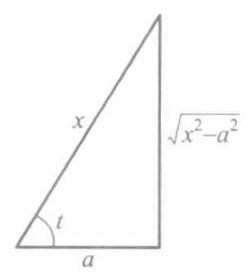
\includegraphics[width=.3\textwidth]{images/P051.jpg}
	\caption{图 $8-2$}
	\label{fig:P051}
\end{figure}

借助图 8-2 的辅助直角三角形,便于求出 \(\sec t = \frac{x}{a},\tan t =\)  \(\frac{\sqrt{{x}^{2} - {a}^{2}}}{a}\) ,故得
\[
\int \frac{\mathrm{d}x}{\sqrt{{x}^{2} - {a}^{2}}} = \ln \left| {\frac{x}{a} + \frac{\sqrt{{x}^{2} - {a}^{2}}}{a}}\right|  + C
\]
\[
= \ln \left| {x + \sqrt{{x}^{2} - {a}^{2}}}\right|  + {C}_{1}\text{ . }
\]
%例 9
\begin{example}

\end{example}
求 \(\int \frac{\mathrm{d}x}{{\left( {x}^{2} + {a}^{2}\right) }^{2}}\left( {a > 0}\right)\) . 解 令 \(x = a\tan t,\left| t\right|  < \frac{\pi }{2}\) (如图 8-3),于是有
\[
\int \frac{\mathrm{d}x}{{\left( {x}^{2} + {a}^{2}\right) }^{2}} = \int \frac{a{\sec }^{2}t}{{a}^{4}{\sec }^{4}t}\mathrm{\;d}t = \frac{1}{{a}^{3}}\int {\cos }^{2}t\mathrm{\;d}t
\]
\[
= \frac{1}{2{a}^{3}}\int \left( {1 + \cos {2t}}\right) \mathrm{d}t
\]
\[
= \frac{1}{2{a}^{3}}\left( {t + \sin t\cos t}\right)  + C
\]
\[
= \frac{1}{2{a}^{3}}\left( {\arctan \frac{x}{a} + \frac{ax}{{x}^{2} + {a}^{2}}}\right)  + C.
\]
\begin{figure}
	\centering
	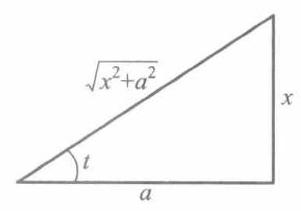
\includegraphics[width=.3\textwidth]{images/P052.jpg}
	\caption{图 $8-3$}
	\label{fig:P052}
\end{figure}

有些不定积分还可采用两种换元方法来计算.

%例 10
\begin{example}

\end{example}
求 \(\int \frac{\mathrm{d}x}{{x}^{2}\sqrt{{x}^{2} - 1}}\) .

%解
\begin{solution}

\end{solution}
解法一 采用第一换元积分法:
\[
\int \frac{\mathrm{d}x}{{x}^{2}\sqrt{{x}^{2} - 1}} = \int \frac{\mathrm{d}x}{{x}^{3}\sqrt{1 - \frac{1}{{x}^{2}}}} = \int \frac{1}{x} \cdot  \frac{-1}{\sqrt{1 - \frac{1}{{x}^{2}}}}\mathrm{\;d}\left( \frac{1}{x}\right)
\]
\[
= \int \frac{-u}{\sqrt{1 - {u}^{2}}}\mathrm{\;d}u = \sqrt{1 - {u}^{2}} + C
\]
\[
= \frac{1}{x}\sqrt{{x}^{2} - 1} + C\text{ . }
\]
解法二 采用第二换元积分法 (令 \(x = \sec t\) ):
\[
\int \frac{\mathrm{d}x}{{x}^{2}\sqrt{{x}^{2} - 1}} = \int \frac{\sec t \cdot  \tan t}{{\sec }^{2}t \cdot  \tan t}\mathrm{\;d}t = \int \cos t\mathrm{\;d}t
\]
\[
= \sin t + C = \frac{1}{x}\sqrt{{x}^{2} - 1} + C.
\]
公式 (1) 与 (2) 分别称为第一换元公式与第二换元公式.

\subsection{分部积分法}

由乘积求导法, 可以导出分部积分法.

%定理 8.6
\begin{theorem}{}{the:}

\end{theorem}
 (分部积分法) 若 \(u\left( x\right)\) 与 \(v\left( x\right)\) 可导,不定积分 \(\int {u}^{\prime }\left( x\right) v\left( x\right) \mathrm{d}x\) 存在,则 \(\int u\left( x\right) {v}^{\prime }\left( x\right) \mathrm{d}x\) 也存在,并有
\[
\int u\left( x\right) {v}^{\prime }\left( x\right) \mathrm{d}x = u\left( x\right) v\left( x\right)  - \int {u}^{\prime }\left( x\right) v\left( x\right) \mathrm{d}x. \tag{3}
\]
%证
\begin{proof}

\end{proof}
由
\[
{\left\lbrack  u\left( x\right) v\left( x\right) \right\rbrack  }^{\prime } = {u}^{\prime }\left( x\right) v\left( x\right)  + u\left( x\right) {v}^{\prime }\left( x\right)
\]
或
\[
u\left( x\right) {v}^{\prime }\left( x\right)  = {\left\lbrack  u\left( x\right) v\left( x\right) \right\rbrack  }^{\prime } - {u}^{\prime }\left( x\right) v\left( x\right) ,
\]
对上式两边求不定积分, 就得到 (3) 式.

公式 (3) 称为分部积分公式, 常简写作
\[
\int u\mathrm{\;d}v = {uv} - \int v\mathrm{\;d}u. \tag{4}
\]
%例 11
\begin{example}

\end{example}
求 \(\int x\cos x\mathrm{\;d}x\) .

%解
\begin{solution}

\end{solution}
令 \(u = x,{v}^{\prime } = \cos x\) ,则有 \({u}^{\prime } = 1,v = \sin x\) . 由公式 (3) 求得
\[
\int x\cos x\mathrm{\;d}x = x\sin x - \int \sin x\mathrm{\;d}x
\]
\[
= x\sin x + \cos x + C\text{ . }
\]
%例 12
\begin{example}

\end{example}
求 \(\int \arctan x\mathrm{\;d}x\) .

%解
\begin{solution}

\end{solution}
令 \(u = \arctan x,{v}^{\prime } = 1\) ,则 \({u}^{\prime } = \frac{1}{1 + {x}^{2}},v = x\) ,由公式 (3) 求得
\[
\int \arctan x\mathrm{\;d}x = x\arctan x - \int \frac{x}{1 + {x}^{2}}\mathrm{\;d}x
\]
\[
= x\arctan x - \frac{1}{2}\ln \left( {1 + {x}^{2}}\right)  + C.
\]
%例 13
\begin{example}

\end{example}
求 \(\int {x}^{3}\ln x\mathrm{\;d}x\) .

%解
\begin{solution}

\end{solution}
令 \(u = \ln x,{v}^{\prime } = {x}^{3}\) ,由公式 (4) 则有
\[
\int {x}^{3}\ln x\mathrm{\;d}x = \int \ln x\mathrm{\;d}\left( \frac{{x}^{4}}{4}\right)  = \frac{1}{4}\left( {{x}^{4}\ln x-\int {x}^{3}\mathrm{\;d}x}\right)
\]
\[
= \frac{{x}^{4}}{16}\left( {4\ln x - 1}\right)  + C.
\]
有时需要接连使用几次分部积分才能求得结果; 有时还会出现与原不定积分同类的项, 需经移项合并后方能完成求解. 现分别示例如下.

%例 14
\begin{example}

\end{example}
求 \(\int {x}^{2}{\mathrm{e}}^{-x}\mathrm{\;d}x\) .

解
\[
\int {x}^{2}{\mathrm{e}}^{-x}\mathrm{\;d}x = \int {x}^{2}\mathrm{\;d}\left( {-{\mathrm{e}}^{-x}}\right)  =  - {x}^{2}{\mathrm{e}}^{-x} + 2\int x{\mathrm{e}}^{-x}\mathrm{\;d}x
\]
\[
=  - {x}^{2}{\mathrm{e}}^{-x} + 2\int x\mathrm{\;d}\left( {-{\mathrm{e}}^{-x}}\right)
\]
\[
=  - {x}^{2}{\mathrm{e}}^{-x} - {2x}{\mathrm{e}}^{-x} + 2\int {\mathrm{e}}^{-x}\mathrm{\;d}x
\]
\[
=  - {\mathrm{e}}^{-x}\left( {{x}^{2} + {2x} + 2}\right)  + C\text{ . }
\]
%例 15
\begin{example}

\end{example}
求 \({I}_{1} = \int {\mathrm{e}}^{ax}\cos {bx}\mathrm{\;d}x\) 和 \({I}_{2} = \int {\mathrm{e}}^{ax}\sin {bx}\mathrm{\;d}x\) .

解
\[
{I}_{1} = \frac{1}{a}\int \cos {bx}\mathrm{\;d}\left( {\mathrm{e}}^{ax}\right)  = \frac{1}{a}\left( {{\mathrm{e}}^{ax}\cos {bx} + b\int {\mathrm{e}}^{ax}\sin {bx}\mathrm{\;d}x}\right)
\]
\[
= \frac{1}{a}\left( {{\mathrm{e}}^{ax}\cos {bx} + b{I}_{2}}\right) ,
\]
\[
{I}_{2} = \frac{1}{a}\int \sin {bx}\mathrm{\;d}\left( {\mathrm{e}}^{ax}\right)  = \frac{1}{a}\left( {{\mathrm{e}}^{ax}\sin {bx} - b{I}_{1}}\right) .
\]
由此得到
\[
\left\{  \begin{array}{l} a{I}_{1} - b{I}_{2} = {\mathrm{e}}^{ax}\cos {bx}, \\  b{I}_{1} + a{I}_{2} = {\mathrm{e}}^{ax}\sin {bx}. \end{array}\right.
\]
解此方程组, 求得
\[
{I}_{1} = \int {\mathrm{e}}^{ax}\cos {bx}\mathrm{\;d}x = {\mathrm{e}}^{ax}\frac{b\sin {bx} + a\cos {bx}}{{a}^{2} + {b}^{2}} + C,
\]
\[
{I}_{2} = \int {\mathrm{e}}^{ax}\sin {bx}\mathrm{\;d}x = {\mathrm{e}}^{ax}\frac{a\sin {bx} - b\cos {bx}}{{a}^{2} + {b}^{2}} + C.
\]
%例 16
\begin{example}

\end{example}
导出不定积分 \({I}_{n} = \int \frac{{x}^{n}}{\sqrt{1 - {x}^{2}}}\mathrm{\;d}x\left( {n\text{ 为正整数 }}\right)\) 的递推公式.

%解
\begin{solution}

\end{solution}
易得 \({I}_{1} =  - \sqrt{1 - {x}^{2}} + C,{I}_{2} = \frac{1}{2}\arcsin x - \frac{1}{2}x\sqrt{1 - {x}^{2}} + C\) . 当 \(n \geq  2\) 时,由分部积分公式, 我们有
\[
{I}_{n} = \int {x}^{n - 1}\mathrm{\;d}\left( {-\sqrt{1 - {x}^{2}}}\right)
\]
\[
=  - {x}^{n - 1}\sqrt{1 - {x}^{2}} + \left( {n - 1}\right) \int {x}^{n - 2}\sqrt{1 - {x}^{2}}\mathrm{\;d}x
\]
\[
=  - {x}^{n - 1}\sqrt{1 - {x}^{2}} + \left( {n - 1}\right) \int \frac{{x}^{n - 2}\left( {1 - {x}^{2}}\right) }{\sqrt{1 - {x}^{2}}}\mathrm{\;d}x
\]
\[
=  - {x}^{n - 1}\sqrt{1 - {x}^{2}} + \left( {n - 1}\right) \int \frac{{x}^{n - 2} - {x}^{n}}{\sqrt{1 - {x}^{2}}}\mathrm{\;d}x
\]
\[
=  - {x}^{n - 1}\sqrt{1 - {x}^{2}} + \left( {n - 1}\right) \int \frac{{x}^{n - 2}}{\sqrt{1 - {x}^{2}}}\mathrm{\;d}x - \left( {n - 1}\right) \int \frac{{x}^{n}}{\sqrt{1 - {x}^{2}}}\mathrm{\;d}x
\]
\[
=  - {x}^{n - 1}\sqrt{1 - {x}^{2}} + \left( {n - 1}\right) {I}_{n - 2} - \left( {n - 1}\right) {I}_{n},
\]
因此得到递推公式
\[
{I}_{n} =  - \frac{1}{n}{x}^{n - 1}\sqrt{1 - {x}^{2}} + \frac{n - 1}{n}{I}_{n - 2}.
\]
\subsection{习题 8.2}

1. 应用换元积分法求下列不定积分:

(1) \(\int \cos \left( {{3x} + 4}\right) \mathrm{d}x\) ;

(2) \(\int x{\mathrm{e}}^{2{x}^{2}}\mathrm{\;d}x\) ；

(3) \(\int \frac{\mathrm{d}x}{{2x} + 1}\) ;

(4) \(\int {\left( 1 + x\right) }^{n}\mathrm{\;d}x\) ;

(5) \(\int \left( {\frac{1}{\sqrt{3 - {x}^{2}}} + \frac{1}{\sqrt{1 - 3{x}^{2}}}}\right) \mathrm{d}x\) ； (6) \(\int {2}^{{2x} + 3}\mathrm{\;d}x\) ;

(7) \(\int \sqrt{8 - {3x}}\mathrm{\;d}x\) ;

(8) \(\int \frac{\mathrm{d}x}{\sqrt[3]{7 - {5x}}}\) ;

(9) \(\int x\sin {x}^{2}\mathrm{\;d}x\) ;

(10) \(\int \frac{\mathrm{d}x}{{\sin }^{2}\left( {{2x} + \frac{\pi }{4}}\right) }\) ;

(11) \(\int \frac{\mathrm{d}x}{1 + \cos x}\) ;

(12) \(\int \frac{\mathrm{d}x}{1 + \sin x}\) ;

(13) \(\int \csc x\mathrm{\;d}x\) ;

(14) \(\int \frac{x}{\sqrt{1 - {x}^{2}}}\mathrm{\;d}x\) ;

(15) \(\int \frac{x}{4 + {x}^{4}}\mathrm{\;d}x\) ;

(16) \(\int \frac{\mathrm{d}x}{x\ln x}\) ;

(17) \(\int \frac{{x}^{4}}{{\left( 1 - {x}^{5}\right) }^{3}}\mathrm{\;d}x\) ;

(18) \(\int \frac{{x}^{3}}{{x}^{8} - 2}\mathrm{\;d}x\) ;

(19) \(\int \frac{\mathrm{d}x}{x\left( {1 + x}\right) }\) ;

(20) \(\int \cot x\mathrm{\;d}x\) ;

(21) \(\int {\cos }^{5}x\mathrm{\;d}x\) ;

(22) \(\int \frac{\mathrm{d}x}{\sin x\cos x}\) ;

(23) \(\int \frac{\mathrm{d}x}{{\mathrm{e}}^{x} + {\mathrm{e}}^{-x}}\) ;

(24) \(\int \frac{{2x} - 3}{{x}^{2} - {3x} + 8}\mathrm{\;d}x\) ;

(25) \(\int \frac{{x}^{2} + 2}{{\left( x + 1\right) }^{3}}\mathrm{\;d}x\) ;

( 26 ) \(\int \frac{\mathrm{d}x}{\sqrt{{x}^{2} + {a}^{2}}}\left( {a > 0}\right)\) ；

( 27 ) \(\int \frac{\mathrm{d}x}{{\left( {x}^{2} + {a}^{2}\right) }^{3/2}}\left( {a > 0}\right)\) ； (28) \(\int \frac{{x}^{5}}{\sqrt{1 - {x}^{2}}}\mathrm{\;d}x\) ;

(29) \(\int \frac{\sqrt{x}}{1 - \sqrt[3]{x}}\mathrm{\;d}x\) ;

(30) \(\int \frac{\sqrt{x + 1} - 1}{\sqrt{x + 1} + 1}\mathrm{\;d}x\) ;

(31) \(\int x{\left( 1 - 2x\right) }^{99}\mathrm{\;d}x\) ;

(32) \(\int \frac{\mathrm{d}x}{x\left( {1 + {x}^{n}}\right) }\left( {n\text{ 为自然数 }}\right)\) ；

(33) \(\int \frac{{x}^{{2n} - 1}}{{x}^{n} + 1}\mathrm{\;d}x\) ;

(34) \(\int \frac{\mathrm{d}x}{x\ln x\ln \ln x}\) ;

(35) \(\int \frac{\ln {2x}}{x\ln {4x}}\mathrm{\;d}x\) ;

( 36 ) \(\int \frac{\mathrm{d}x}{{x}^{4}\sqrt{{x}^{2} - 1}}\) .

2. 应用分部积分法求下列不定积分:

(1) \(\int \arcsin x\mathrm{\;d}x\) ;

(2) \(\int \ln x\mathrm{\;d}x\) ;

(3) \(\int {x}^{2}\cos x\mathrm{\;d}x\) ;

(4) \(\int \frac{\ln x}{{x}^{3}}\mathrm{\;d}x\) ;

(5) \(\int {\left( \ln x\right) }^{2}\mathrm{\;d}x\) ;

(6) \(\int x\arctan x\mathrm{\;d}x\) ;

(7) \(\int \left\lbrack  {\ln \left( {\ln x}\right)  + \frac{1}{\ln x}}\right\rbrack  \mathrm{d}x\) ;

(8) \(\int {\left( \arcsin x\right) }^{2}\mathrm{\;d}x\) ;

(9) \(\int {\sec }^{3}x\mathrm{\;d}x\) ;

( 10 ) \(\int \sqrt{{x}^{2} \pm  {a}^{2}}\mathrm{\;d}x\left( {a > 0}\right)\) .

3. 求下列不定积分:

(1) \(\int {\left\lbrack  f\left( x\right) \right\rbrack  }^{\alpha }{f}^{\prime }\left( x\right) \mathrm{d}x\left( {\alpha  \neq   - 1}\right)\) ;

(2) \(\int \frac{{f}^{\prime }\left( x\right) }{1 + {\left\lbrack  f\left( x\right) \right\rbrack  }^{2}}\mathrm{\;d}x\) ;

(3) \(\int \frac{{f}^{\prime }\left( x\right) }{f\left( x\right) }\mathrm{d}x\) ;

(4) \(\int {\mathrm{e}}^{f\left( x\right) }{f}^{\prime }\left( x\right) \mathrm{d}x\) .

4. 证明:

(1)若 \({I}_{n} = \int {\tan }^{n}x\mathrm{\;d}x,n = 2,3,\cdots\) ,则
\[
{I}_{n} = \frac{1}{n - 1}{\tan }^{n - 1}x - {I}_{n - 2}.
\]
(2)若 \(I\left( {m,n}\right)  = \int {\cos }^{m}x{\sin }^{n}x\mathrm{\;d}x\) ,则当 \(m + n \neq  0\) 时,
\[
I\left( {m,n}\right)  = \frac{{\cos }^{m - 1}x{\sin }^{n + 1}x}{m + n} + \frac{m - 1}{m + n}I\left( {m - 2,n}\right)
\]
\[
=  - \frac{{\cos }^{m + 1}x{\sin }^{n - 1}x}{m + n} + \frac{n - 1}{m + n}I\left( {m,n - 2}\right) ,
\]
\[
n,m = 2,3,\cdots \text{ . }
\]
5. 利用上题的递推公式计算:

(1) \(\int {\tan }^{3}x\mathrm{\;d}x\) ;

(2) \(\int {\tan }^{4}x\mathrm{\;d}x\) ;

(3) \(\int {\cos }^{2}x{\sin }^{4}x\mathrm{\;d}x\) .

6. 导出下列不定积分对于正整数 \(n\) 的递推公式:

(1) \({I}_{n} = \int {x}^{n}{\mathrm{e}}^{kx}\mathrm{\;d}x\) ;

(2) \({I}_{n} = \int {\left( \ln x\right) }^{n}\mathrm{\;d}x\) ;

(3) \({I}_{n} = \int {\left( \arcsin x\right) }^{n}\mathrm{\;d}x\) ;

(4) \({I}_{n} = \int {\mathrm{e}}^{ax}{\sin }^{n}x\mathrm{\;d}x\) .

7. 利用上题所得递推公式计算:

(1) \(\int {x}^{3}{\mathrm{e}}^{2x}\mathrm{\;d}x\) ;

(2) \(\int {\left( \ln x\right) }^{3}\mathrm{\;d}x\) ;

(3) \(\int {\left( \arcsin x\right) }^{3}\mathrm{\;d}x\) ;

(4) \(\int {\mathrm{e}}^{x}{\sin }^{3}x\mathrm{\;d}x\) .

\section{有理函数和可化为有理函数的不定积分}

至此我们已经学得了一些最基本的积分方法. 在此基础上, 本节将讨论某些特殊类型的不定积分, 这些不定积分无论怎样复杂, 原则上都可按一定的步骤把它求出来.

\subsection{有理函数的不定积分}

有理函数是指由两个多项式函数的商所表示的函数, 其一般形式为
\[
R\left( x\right)  = \frac{P\left( x\right) }{Q\left( x\right) } = \frac{{\alpha }_{0}{x}^{n} + {\alpha }_{1}{x}^{n - 1} + \cdots  + {\alpha }_{n}}{{\beta }_{0}{x}^{m} + {\beta }_{1}{x}^{m - 1} + \cdots  + {\beta }_{m}}, \tag{1}
\]
其中 \(n,m\) 为非负整数, \({\alpha }_{0},{\alpha }_{1},\cdots ,{\alpha }_{n}\) 与 \({\beta }_{0},{\beta }_{1},\cdots ,{\beta }_{m}\) 都是常数,且 \({\alpha }_{0} \neq  0,{\beta }_{0} \neq  0\) . 若 \(m >\)  \(n\) ,则称它为真分式; 若 \(m \leq  n\) ,则称它为假分式. 由多项式的除法可知,假分式总能化为一个多项式与一个真分式之和. 由于多项式的不定积分是容易求得的, 因此只需研究真分式的不定积分, 故设 (1) 为一有理真分式.

根据代数知识,如果多项式 \({Q}_{1}\left( x\right)\) 与 \({Q}_{2}\left( x\right)\) 是互素的,即 \(\left( {{Q}_{1}\left( x\right) ,{Q}_{2}\left( x\right) }\right)  = 1\) ,则存在多项式 \({P}_{1}\left( x\right)\) 与 \({P}_{2}\left( x\right)\) ,使得 \({P}_{1}\left( x\right) {Q}_{1}\left( x\right)  + {P}_{2}\left( x\right) {Q}_{2}\left( x\right)  = 1\) . 于是
\[
\frac{1}{{Q}_{1}\left( x\right) {Q}_{2}\left( x\right) } = \frac{{P}_{1}\left( x\right) {Q}_{1}\left( x\right)  + {P}_{2}\left( x\right) {Q}_{2}\left( x\right) }{{Q}_{1}\left( x\right) {Q}_{2}\left( x\right) } = \frac{{P}_{1}\left( x\right) }{{Q}_{2}\left( x\right) } + \frac{{P}_{2}\left( x\right) }{{Q}_{1}\left( x\right) }
\]
因此, 有理真分式必定可以表示成若干个部分分式之和 (称为部分分式分解). 因而问题归结为求那些部分分式的不定积分. 为此, 先把怎样分解部分分式的步骤简述如下 (可与后面的例 1 对照着做):

第一步 对分母 \(Q\left( x\right)\) 在实系数内作标准分解:
\[
Q\left( x\right)  = {\left( x - {a}_{1}\right) }^{{\lambda }_{1}}\cdots {\left( x - {a}_{s}\right) }^{{\lambda }_{s}}{\left( {x}^{2} + {p}_{1}x + {q}_{1}\right) }^{{\mu }_{1}}\cdots {\left( {x}^{2} + {p}_{t}x + {q}_{t}\right) }^{{\mu }_{t}}, \tag{2}
\]
其中 \({\beta }_{0} = 1,{\lambda }_{i},{\mu }_{j}\left( {i = 1,2,\cdots ,s;j = 1,2,\cdots ,t}\right)\) 均为自然数,而且
\[
\mathop{\sum }\limits_{{i = 1}}^{s}{\lambda }_{i} + 2\mathop{\sum }\limits_{{j = 1}}^{t}{\mu }_{j} = m;\;{p}_{j}^{2} - 4{q}_{j} < 0,\;j = 1,2,\cdots ,t.
\]
第二步 根据分母的各个因式分别写出与之相应的部分分式: 对于每个形如 \((x -\)  \(a{)}^{k}\) 的因式,它所对应的部分分式是
\[
\frac{{A}_{1}}{x - a} + \frac{{A}_{2}}{{\left( x - a\right) }^{2}} + \cdots  + \frac{{A}_{k}}{{\left( x - a\right) }^{k}};
\]
对每个形如 \({\left( {x}^{2} + px + q\right) }^{k}\) 的因式,它所对应的部分分式是
\[
\frac{{B}_{1}x + {C}_{1}}{{x}^{2} + {px} + q} + \frac{{B}_{2}x + {C}_{2}}{{\left( {x}^{2} + px + q\right) }^{2}} + \cdots  + \frac{{B}_{k}x + {C}_{k}}{{\left( {x}^{2} + px + q\right) }^{k}}.
\]
把所有部分分式加起来,使之等于 \(R\left( x\right)\) . (至此,部分分式中的常数系数 \({A}_{i},{B}_{i},{C}_{i}\) 尚为待定的.)

第三步 确定待定系数:一般方法是将所有部分分式通分相加, 所得分式的分母即为原分母 \(Q\left( x\right)\) ,而其分子亦应与原分子 \(P\left( x\right)\) 恒等. 于是,按同幂项系数必定相等, 得到一组关于待定系数的线性方程, 这组方程的解就是需要确定的系数.

%例 1
\begin{example}

\end{example}
对 \(R\left( x\right)  = \frac{2{x}^{4} - {x}^{3} + 4{x}^{2} + {9x} - {10}}{{x}^{5} + {x}^{4} - 5{x}^{3} - 2{x}^{2} + {4x} - 8}\) 作部分分式分解.

%解
\begin{solution}

\end{solution}
按上述步骤依次执行如下:
\[
Q\left( x\right)  = {x}^{5} + {x}^{4} - 5{x}^{3} - 2{x}^{2} + {4x} - 8
\]
\[
= \left( {x - 2}\right) {\left( x + 2\right) }^{2}\left( {{x}^{2} - x + 1}\right) \text{ . }
\]
部分分式分解的待定形式为
\[
R\left( x\right)  = \frac{{A}_{0}}{x - 2} + \frac{{A}_{1}}{x + 2} + \frac{{A}_{2}}{{\left( x + 2\right) }^{2}} + \frac{{Bx} + C}{{x}^{2} - x + 1}. \tag{3}
\]
用 \(Q\left( x\right)\) 乘上式两边,得一恒等式
\[
2{x}^{4} - {x}^{3} + 4{x}^{2} + {9x} - {10} \equiv  {A}_{0}{\left( x + 2\right) }^{2}\left( {{x}^{2} - x + 1}\right)  +
\]
\[
{A}_{1}\left( {x - 2}\right) \left( {x + 2}\right) \left( {{x}^{2} - x + 1}\right)  + {A}_{2}\left( {x - 2}\right) \left( {{x}^{2} - x + 1}\right)  +
\]
\[
\left( {{Bx} + C}\right) \left( {x - 2}\right) {\left( x + 2\right) }^{2}. \tag{4}
\]
然后使等式两边同幂项系数相等, 得到线性方程组:
\[
\left\{  \begin{array}{l} {A}_{0} + {A}_{1} + B = 2, \\  3{A}_{0} - {A}_{1} + {A}_{2} + {2B} + C =  - 1,\cdots \cdots \cdots \cdots \cdots \cdots \cdots \cdots {x}^{3}\text{ 的系数 } \\  {A}_{0} - 3{A}_{1} - 3{A}_{2} - {4B} + {2C} = 4,\cdots \cdots \cdots \cdots \cdots \cdots \cdots {x}^{2}\text{ 的系数 } \\  4{A}_{1} + 3{A}_{2} - {8B} - {4C} = 9,\cdots \cdots \cdots \cdots \cdots \cdots \cdots \cdots \cdots \cdots x\text{ 的系数 } \\  4{A}_{0} - 4{A}_{1} - 2{A}_{2} - {8C} =  - {10}.\cdots \cdots \cdots \cdots \cdots \cdots \cdots \cdots \text{ 常数项 } \end{array}\right.
\]
求出它的解: \({A}_{0} = 1,{A}_{1} = 2,{A}_{2} =  - 1,B =  - 1,C = 1\) ,并代入 (3) 式,这便完成了对 \(R\left( x\right)\) 的部分分式分解:
\[
R\left( x\right)  = \frac{1}{x - 2} + \frac{2}{x + 2} - \frac{1}{{\left( x + 2\right) }^{2}} - \frac{x - 1}{{x}^{2} - x + 1}.
\]
上述待定系数法有时可用较简便的方法去替代. 例如可将 \(x\) 的某些特定值 (如 \(Q\left( x\right)  = 0\) 的根) 代入 (4) 式,以便得到一组较简单的方程,或直接求得某几个待定系数的值. 对于上例,若分别用 \(x = 2\) 和 \(x =  - 2\) 代入 (4) 式,立即求得
\[
{A}_{0} = 1\text{ 和 }{A}_{2} =  - 1.
\]
于是 (4) 式简化成为
\[
{x}^{4} - 3{x}^{3} + {12x} - {16} = {A}_{1}\left( {x - 2}\right) \left( {x + 2}\right) \left( {{x}^{2} - x + 1}\right)  +
\]
\[
\left( {{Bx} + C}\right) \left( {x - 2}\right) {\left( x + 2\right) }^{2}.
\]
为继续求得 \({A}_{1},B,C\) ,还可用 \(x\) 的三个简单值代入上式,如令 \(x = 0,1, - 1\) ,相应得到
\[
\left\{  \begin{array}{l} {A}_{1} + {2C} = 4, \\  {A}_{1} + {3B} + {3C} = 2, \\  3{A}_{1} - B + C = 8. \end{array}\right.
\]
由此易得 \({A}_{1} = 2,B =  - 1,C = 1\) . 这就同样确定了所有待定系数.

一旦完成了部分分式分解, 最后求各个部分分式的不定积分. 由以上讨论知道, 任何有理真分式的不定积分都将归为求以下两种形式的不定积分:

( I ) \(\int \frac{\mathrm{d}x}{{\left( x - a\right) }^{k}}\) ;

( II ) \(\int \frac{{Lx} + M}{{\left( {x}^{2} + px + q\right) }^{k}}\mathrm{\;d}x\left( {{p}^{2} - {4q} < 0}\right)\) .

对于(I),已知
\[
\int \frac{\mathrm{d}x}{{\left( x - a\right) }^{k}} = \left\{  \begin{matrix} \ln \left| {x - a}\right|  + C, & k = 1, \\  \frac{1}{\left( {1 - k}\right) {\left( x - a\right) }^{k - 1}} + C, & k > 1. \end{matrix}\right.
\]
对于 (II),只要作适当换元 \(\left( {\text{ 令 }t = x + \frac{p}{2}}\right)\) ,便化为
\[
\int \frac{{Lx} + M}{{\left( {x}^{2} + px + q\right) }^{k}}\mathrm{\;d}x = \int \frac{{Lt} + N}{{\left( {t}^{2} + {r}^{2}\right) }^{k}}\mathrm{\;d}t
\]
\[
= L\int \frac{t}{{\left( {t}^{2} + {r}^{2}\right) }^{k}}\mathrm{\;d}t + N\int \frac{\mathrm{d}t}{{\left( {t}^{2} + {r}^{2}\right) }^{k}}, \tag{5}
\]
其中 \({r}^{2} = q - \frac{{p}^{2}}{4},N = M - \frac{p}{2}L\) .

当 \(k = 1\) 时,(5) 式右边两个不定积分分别为
\[
\int \frac{t}{{t}^{2} + {r}^{2}}\mathrm{\;d}t = \frac{1}{2}\ln \left( {{t}^{2} + {r}^{2}}\right)  + C,
\]
\[
\int \frac{\mathrm{d}t}{{t}^{2} + {r}^{2}} = \frac{1}{r}\arctan \frac{t}{r} + C. \tag{6}
\]
当 \(k \geq  2\) 时,(5) 式右边第一个不定积分为
\[
\int \frac{t}{{\left( {t}^{2} + {r}^{2}\right) }^{k}}\mathrm{\;d}t = \frac{1}{2\left( {1 - k}\right) {\left( {t}^{2} + {r}^{2}\right) }^{k - 1}} + C.
\]
对于第二个不定积分, 记
\[
{I}_{k} = \int \frac{\mathrm{d}t}{{\left( {t}^{2} + {r}^{2}\right) }^{k}},
\]
可用分部积分法导出递推公式如下:
\[
{I}_{k} = \frac{1}{{r}^{2}}\int \frac{\left( {{t}^{2} + {r}^{2}}\right)  - {t}^{2}}{{\left( {t}^{2} + {r}^{2}\right) }^{k}}\mathrm{\;d}t
\]
\[
= \frac{1}{{r}^{2}}{I}_{k - 1} - \frac{1}{{r}^{2}}\int \frac{{t}^{2}}{{\left( {t}^{2} + {r}^{2}\right) }^{k}}\mathrm{\;d}t
\]
\[
= \frac{1}{{r}^{2}}{I}_{k - 1} + \frac{1}{2{r}^{2}\left( {k - 1}\right) }\int t\mathrm{\;d}\left( \frac{1}{{\left( {t}^{2} + {r}^{2}\right) }^{k - 1}}\right)
\]
\[
= \frac{1}{{r}^{2}}{I}_{k - 1} + \frac{1}{2{r}^{2}\left( {k - 1}\right) }\left\lbrack  {\frac{t}{{\left( {t}^{2} + {r}^{2}\right) }^{k - 1}} - {I}_{k - 1}}\right\rbrack  .
\]
经整理得到
\[
{I}_{k} = \frac{t}{2{r}^{2}\left( {k - 1}\right) {\left( {t}^{2} + {r}^{2}\right) }^{k - 1}} + \frac{{2k} - 3}{2{r}^{2}\left( {k - 1}\right) }{I}_{k - 1}. \tag{7}
\]
重复使用递推公式 (7),最终归为计算 \({I}_{1}\) ,这已由 (6) 式给出.

把所有这些局部结果代回 (5) 式,并令 \(t = x + \frac{p}{2}\) ,就完成了对不定积分 (II) 的计算.

%例 2
\begin{example}

\end{example}
求 \(\int \frac{{x}^{2} + 1}{{\left( {x}^{2} - 2x + 2\right) }^{2}}\mathrm{\;d}x\) .

%解
\begin{solution}

\end{solution}
在本题中, 由于被积函数的分母只有单一因式, 因此, 部分分式分解能被简化为
\[
\frac{{x}^{2} + 1}{{\left( {x}^{2} - 2x + 2\right) }^{2}} = \frac{\left( {{x}^{2} - {2x} + 2}\right)  + \left( {{2x} - 1}\right) }{{\left( {x}^{2} - 2x + 2\right) }^{2}}
\]
\[
= \frac{1}{{x}^{2} - {2x} + 2} + \frac{{2x} - 1}{{\left( {x}^{2} - 2x + 2\right) }^{2}}\text{ . }
\]
现分别计算部分分式的不定积分如下:
\[
\int \frac{\mathrm{d}x}{{x}^{2} - {2x} + 2} = \int \frac{\mathrm{d}\left( {x - 1}\right) }{{\left( x - 1\right) }^{2} + 1} = \arctan \left( {x - 1}\right)  + {C}_{1}.
\]
\[
\int \frac{{2x} - 1}{{\left( {x}^{2} - 2x + 2\right) }^{2}}\mathrm{\;d}x = \int \frac{\left( {{2x} - 2}\right)  + 1}{{\left( {x}^{2} - 2x + 2\right) }^{2}}\mathrm{\;d}x
\]
\[
= \int \frac{\mathrm{d}\left( {{x}^{2} - {2x} + 2}\right) }{{\left( {x}^{2} - 2x + 2\right) }^{2}} + \int \frac{\mathrm{d}\left( {x - 1}\right) }{{\left\lbrack  {\left( x - 1\right) }^{2} + 1\right\rbrack  }^{2}}
\]
\[
= \frac{-1}{{x}^{2} - {2x} + 2} + \int \frac{\mathrm{d}t}{{\left( {t}^{2} + 1\right) }^{2}}.
\]
由递推公式 (7), 求得其中
\[
\int \frac{\mathrm{d}t}{{\left( {t}^{2} + 1\right) }^{2}} = \frac{t}{2\left( {{t}^{2} + 1}\right) } + \frac{1}{2}\int \frac{\mathrm{d}t}{{t}^{2} + 1}
\]
\[
= \frac{x - 1}{2\left( {{x}^{2} - {2x} + 2}\right) } + \frac{1}{2}\arctan \left( {x - 1}\right)  + {C}_{2}.
\]
于是得到
\[
\int \frac{{x}^{2} + 1}{{\left( {x}^{2} - 2x + 2\right) }^{2}}\mathrm{\;d}x = \frac{x - 3}{2\left( {{x}^{2} - {2x} + 2}\right) } + \frac{3}{2}\arctan \left( {x - 1}\right)  + C.
\]
下面再介绍几类被积函数能变换为有理函数的不定积分.

\subsection{三角函数有理式的不定积分}

由 \(u\left( x\right) ,v\left( x\right)\) 及常数经过有限次四则运算所得到的函数称为关于 \(u\left( x\right) ,v\left( x\right)\) 的有理式,并用 \(R\left( {u\left( x\right) ,v\left( x\right) }\right)\) 表示.

\(\int R\left( {\sin x,\cos x}\right) \mathrm{d}x\) 是三角函数有理式的不定积分.一般通过变换 \(t = \tan \frac{x}{2}\) ,可把它化为有理函数的不定积分. 这是因为
\[
\sin x = \frac{2\sin \frac{x}{2}\cos \frac{x}{2}}{{\sin }^{2}\frac{x}{2} + {\cos }^{2}\frac{x}{2}} = \frac{2\tan \frac{x}{2}}{1 + {\tan }^{2}\frac{x}{2}} = \frac{2t}{1 + {t}^{2}}, \tag{8}
\]
\[
\cos x = \frac{{\cos }^{2}\frac{x}{2} - {\sin }^{2}\frac{x}{2}}{{\sin }^{2}\frac{x}{2} + {\cos }^{2}\frac{x}{2}} = \frac{1 - {\tan }^{2}\frac{x}{2}}{1 + {\tan }^{2}\frac{x}{2}} = \frac{1 - {t}^{2}}{1 + {t}^{2}}, \tag{9}
\]
\[
\mathrm{d}x = \frac{2}{1 + {t}^{2}}\mathrm{\;d}t, \tag{10}
\]
所以 \(\int R\left( {\sin x,\cos x}\right) \mathrm{d}x = \int R\left( {\frac{2t}{1 + {t}^{2}},\frac{1 - {t}^{2}}{1 + {t}^{2}}}\right) \frac{2}{1 + {t}^{2}}\mathrm{\;d}t\) .

%例 3
\begin{example}

\end{example}
求 \(\int \frac{1 + \sin x}{\sin x\left( {1 + \cos x}\right) }\mathrm{d}x\) .

%解
\begin{solution}

\end{solution}
令 \(t = \tan \frac{x}{2}\) ,将 (8)、(9)、(10)代入被积表达式,
\[
\int \frac{1 + \sin x}{\sin x\left( {1 + \cos x}\right) }\mathrm{d}x = \int \frac{1 + \frac{2t}{1 + {t}^{2}}}{\frac{2t}{1 + {t}^{2}}\left( {1 + \frac{1 - {t}^{2}}{1 + {t}^{2}}}\right) } \cdot  \frac{2}{1 + {t}^{2}}\mathrm{\;d}t
\]
\[
= \int \frac{1}{2}\left( {t + 2 + \frac{1}{t}}\right) \mathrm{d}t = \frac{1}{2}\left( {\frac{{t}^{2}}{2} + {2t} + \ln \left| t\right| }\right)  + C
\]
\[
= \frac{1}{4}{\tan }^{2}\frac{x}{2} + \tan \frac{x}{2} + \frac{1}{2}\ln \left| {\tan \frac{x}{2}}\right|  + C.
\]
注意 上面所用的变换 \(t = \tan \frac{x}{2}\) 对三角函数有理式的不定积分虽然总是有效的, 但并不意味着在任何场合都是简便的.

%例 4
\begin{example}

\end{example}
求 \(\int \frac{\mathrm{d}x}{{a}^{2}{\sin }^{2}x + {b}^{2}{\cos }^{2}x}\left( {{ab} \neq  0}\right)\) .

%解
\begin{solution}

\end{solution}
由于
\[
\int \frac{\mathrm{d}x}{{a}^{2}{\sin }^{2}x + {b}^{2}{\cos }^{2}x} = \int \frac{{\sec }^{2}x}{{a}^{2}{\tan }^{2}x + {b}^{2}}\mathrm{\;d}x = \int \frac{\mathrm{d}\left( {\tan x}\right) }{{a}^{2}{\tan }^{2}x + {b}^{2}},
\]
故令 \(t = \tan x\) ,就有
\[
\int \frac{\mathrm{d}x}{{a}^{2}{\sin }^{2}x + {b}^{2}{\cos }^{2}x} = \int \frac{\mathrm{d}t}{{a}^{2}{t}^{2} + {b}^{2}} = \frac{1}{a}\int \frac{\mathrm{d}\left( {at}\right) }{{\left( at\right) }^{2} + {b}^{2}}
\]
\[
= \frac{1}{ab}\arctan \frac{at}{b} + C
\]
\[
= \frac{1}{ab}\arctan \left( {\frac{a}{b}\tan x}\right)  + C.
\]
通常当被积函数是 \({\sin }^{2}x,{\cos }^{2}x\) 及 \(\sin x\cos x\) 的有理式时,采用变换 \(t = \tan x\) 往往较为简便. 其他特殊情形可因题而异, 选择合适的变换.

\subsection{某些无理根式的不定积分}

1. \(\int R\left( {x,\sqrt[n]{\frac{{ax} + b}{{cx} + d}}}\right) \mathrm{d}x\) 型不定积分 \(\left( {{ad} - {bc} \neq  0}\right)\) . 对此只需令 \(t = \sqrt[n]{\frac{{ax} + b}{{cx} + d}}\) ,就可化为有理函数的不定积分.

%例 5
\begin{example}

\end{example}
求 \(\int \frac{1}{x}\sqrt{\frac{x + 2}{x - 2}}\mathrm{\;d}x\) .

%解
\begin{solution}

\end{solution}
令 \(t = \sqrt{\frac{x + 2}{x - 2}}\) ,则有 \(x = \frac{2\left( {{t}^{2} + 1}\right) }{{t}^{2} - 1},\mathrm{\;d}x = \frac{-{8t}}{{\left( {t}^{2} - 1\right) }^{2}}\mathrm{\;d}t\) ,
\[
\int \frac{1}{x}\sqrt{\frac{x + 2}{x - 2}}\mathrm{\;d}x = \int \frac{4{t}^{2}}{\left( {1 - {t}^{2}}\right) \left( {1 + {t}^{2}}\right) }\mathrm{d}t
\]
\[
= \int \left( {\frac{2}{1 - {t}^{2}} - \frac{2}{1 + {t}^{2}}}\right) \mathrm{d}t
\]
\[
= \ln \left| \frac{1 + t}{1 - t}\right|  - 2\arctan t + C
\]
\[
= \ln \left| \frac{1 + \sqrt{\left( {x + 2}\right) /\left( {x - 2}\right) }}{1 - \sqrt{\left( {x + 2}\right) /\left( {x - 2}\right) }}\right|  - 2\arctan \sqrt{\frac{x + 2}{x - 2}} + C.
\]
%例 6
\begin{example}

\end{example}
求 \(\int \frac{\mathrm{d}x}{\left( {1 + x}\right) \sqrt{2 + x - {x}^{2}}}\) .

%解
\begin{solution}

\end{solution}
由于
\[
\frac{1}{\left( {1 + x}\right) \sqrt{2 + x - {x}^{2}}} = \frac{1}{{\left( 1 + x\right) }^{2}}\sqrt{\frac{1 + x}{2 - x}},
\]
故令 \(t = \sqrt{\frac{1 + x}{2 - x}}\) ,则有 \(x = \frac{2{t}^{2} - 1}{1 + {t}^{2}},\mathrm{\;d}x = \frac{6t}{{\left( 1 + {t}^{2}\right) }^{2}}\mathrm{\;d}t\) ,
\[
\int \frac{\mathrm{d}x}{\left( {1 + x}\right) \sqrt{2 + x - {x}^{2}}} = \int \frac{1}{{\left( 1 + x\right) }^{2}}\sqrt{\frac{1 + x}{2 - x}}\mathrm{\;d}x
\]
\[
= \int \frac{{\left( 1 + {t}^{2}\right) }^{2}}{9{t}^{4}} \cdot  t \cdot  \frac{6t}{{\left( 1 + {t}^{2}\right) }^{2}}\mathrm{\;d}t = \int \frac{2}{3{t}^{2}}\mathrm{\;d}t
\]
\[
=  - \frac{2}{3t} + C =  - \frac{2}{3}\sqrt{\frac{2 - x}{1 + x}} + C.
\]
2. \(\int R\left( {x,\sqrt{a{x}^{2} + {bx} + c}}\right) \mathrm{d}x\) 型不定积分 \(\left( {a > 0}\right.\) 时 \(\left. {{b}^{2} - {4ac} \neq  0,a < 0\text{ 时 }{b}^{2} - {4ac} > 0}\right)\) .

由于
\[
a{x}^{2} + {bx} + c = a\left\lbrack  {{\left( x + \frac{b}{2a}\right) }^{2} + \frac{{4ac} - {b}^{2}}{4{a}^{2}}}\right\rbrack  ,
\]
若记 \(u = x + \frac{b}{2a},{k}^{2} = \left| \frac{{4ac} - {b}^{2}}{4{a}^{2}}\right|\) ,则此二次三项式必属于以下三种情形之一:
\[
\left| a\right| \left( {{u}^{2} + {k}^{2}}\right) ,\left| a\right| \left( {{u}^{2} - {k}^{2}}\right) ,\left| a\right| \left( {{k}^{2} - {u}^{2}}\right) .
\]
因此上述无理根式的不定积分也就转化为以下三种类型之一:
\[
\int R\left( {u,\sqrt{{u}^{2} \pm  {k}^{2}}}\right) \mathrm{d}u,\;\int R\left( {u,\sqrt{{k}^{2} - {u}^{2}}}\right) \mathrm{d}u.
\]
当分别令 \(u = k\tan t,u = k\sec t,u = k\sin t\) 后,它们都化为三角有理式的不定积分.

%例 7
\begin{example}

\end{example}
求 \(I = \int \frac{\mathrm{d}x}{x\sqrt{{x}^{2} - {2x} - 3}}\) .

%解
\begin{solution}

\end{solution}
解法一 按上述一般步骤, 求得
\[
I = \int \frac{\mathrm{d}x}{x\sqrt{{\left( x - 1\right) }^{2} - 4}} = \int \frac{\mathrm{d}u}{\left( {u + 1}\right) \sqrt{{u}^{2} - 4}}
\]
\[
= \int \frac{2\sec \theta \tan \theta }{\left( {2\sec \theta  + 1}\right)  \cdot  2\tan \theta }\mathrm{d}\theta
\]
181
\[
= \int \frac{\mathrm{d}\theta }{2 + \cos \theta } = \int \frac{\frac{2}{1 + {t}^{2}}}{2 + \frac{1 - {t}^{2}}{1 + {t}^{2}}}\mathrm{\;d}t
\]
\[
\left( {t = \tan \frac{\theta }{2}}\right)
\]
\[
= \int \frac{2}{{t}^{2} + 3}\mathrm{\;d}t = \frac{2}{\sqrt{3}}\arctan \frac{t}{\sqrt{3}} + C
\]
\[
= \frac{2}{\sqrt{3}}\arctan \left( {\frac{1}{\sqrt{3}}\tan \frac{\theta }{2}}\right)  + C.
\]
由于
\[
\tan \frac{\theta }{2} = \frac{\sin \theta }{1 + \cos \theta } = \frac{\tan \theta }{\sec \theta  + 1}
\]
\[
= \frac{\sqrt{{\left( \frac{u}{2}\right) }^{2} - 1}}{\frac{u}{2} + 1} = \frac{\sqrt{{x}^{2} - {2x} - 3}}{x + 1},
\]
因此
\[
I = \frac{2}{\sqrt{3}}\arctan \frac{\sqrt{{x}^{2} - {2x} - 3}}{\sqrt{3}\left( {x + 1}\right) } + C.
\]
解法二 若令 \(\sqrt{{x}^{2} - {2x} - 3} = x - t\) ,则可解出
\[
x = \frac{{t}^{2} + 3}{2\left( {t - 1}\right) },\;\mathrm{d}x = \frac{{t}^{2} - {2t} - 3}{2{\left( t - 1\right) }^{2}}\mathrm{\;d}t,
\]
\[
\sqrt{{x}^{2} - {2x} - 3} = \frac{{t}^{2} + 3}{2\left( {t - 1}\right) } - t = \frac{-\left( {{t}^{2} - {2t} - 3}\right) }{2\left( {t - 1}\right) }.
\]
于是所求不定积分直接化为有理函数的不定积分:
\[
I = \int \frac{2\left( {t - 1}\right) }{{t}^{2} + 3} \cdot  \frac{2\left( {t - 1}\right) }{-\left( {{t}^{2} - {2t} - 3}\right) } \cdot  \frac{{t}^{2} - {2t} - 3}{2{\left( t - 1\right) }^{2}}\mathrm{\;d}t
\]
\[
=  - \int \frac{2}{{t}^{2} + 3}\mathrm{\;d}t =  - \frac{2}{\sqrt{3}}\arctan \frac{t}{\sqrt{3}} + C
\]
\[
= \frac{2}{\sqrt{3}}\arctan \frac{\sqrt{{x}^{2} - {2x} - 3} - x}{\sqrt{3}} + C.
\]
%注
\begin{remark}

\end{remark}
1 可以证明
\[
\arctan \frac{\sqrt{{x}^{2} - {2x} - 3} - x}{\sqrt{3}} = \arctan \frac{\sqrt{{x}^{2} - {2x} - 3}}{\sqrt{3}\left( {x + 1}\right) } - \frac{\pi }{3},
\]
所以两种解法所得结果是一致的. 此外,上述结果对 \(x < 0\) 同样成立.

%注
\begin{remark}

\end{remark}
2 相比之下, 解法二优于解法一. 这是因为它所选择的变换能直接化为有理形式 (而解法一通过三次换元才化为有理形式). 如果改令
\[
\sqrt{{x}^{2} - {2x} - 3} = x + t,
\]
显然有相同效果——两边各自平方后能消去 \({x}^{2}\) 项,从而解出 \(x\) 为 \(t\) 的有理函数.

一般地,二次三项式 \(a{x}^{2} + {bx} + c\) 中,若 \(a > 0\) ,则可令
\[
\sqrt{a{x}^{2} + {bx} + c} = \sqrt{a}x \pm  t;
\]
若 \(c > 0\) ,还可令
\[
\sqrt{a{x}^{2} + {bx} + c} = {xt} \pm  \sqrt{c}.
\]
这类变换称为欧拉变换.

至此我们已经学过了求不定积分的基本方法, 以及某些特殊类型不定积分的求法. 需要指出的是, 通常所说的 “求不定积分”, 是指用初等函数的形式把这个不定积分表示出来. 在这个意义下, 并不是任何初等函数的不定积分都能 “求出” 来的. 例如:
\[
\int {\mathrm{e}}^{\pm {x}^{2}}\mathrm{\;d}x,\int \frac{\mathrm{d}x}{\ln x},\int \frac{\sin x}{x}\mathrm{\;d}x,\int \sqrt{1 - {k}^{2}{\sin }^{2}x}\mathrm{\;d}x\left( {0 < {k}^{2} < 1}\right) ,
\]
等等, 虽然它们都存在, 但却无法用初等函数来表示 (这个结论证明起来是非常难的, 刘维尔 (Liouville) 于 1835 年作出过证明). 因此可以说, 初等函数的原函数不一定是初等函数. 在下一章将会知道, 这类非初等函数可采用定积分形式来表示.

最后顺便指出, 在求不定积分时, 还可利用现成的积分表. 在积分表中所有的积分公式是按被积函数分类编排的, 人们只要根据被积函数的类型, 或经过适当变形化为表中列出的类型, 查阅公式即可.此外, 有些计算器 (例如 TI-92 型) 和电脑软件 (例如 Mathemetica, Maple 等) 也都具有求不定积分的实用功能. 但对于初学者来说, 首先应该掌握各种基本的积分方法.

在附录 II 中列出了一份容量不大的积分表, 它大体上是典型例题和习题的总结. 列出这份积分表的主要目的是为大家学习后继课程提供方便.

\subsection{习题 8.3}

1. 求下列不定积分:

(1) \(\int \frac{{x}^{3}}{x - 1}\mathrm{\;d}x\) ;

(2) \(\int \frac{x - 2}{{x}^{2} - {7x} + {12}}\mathrm{\;d}x\) ；

(3) \(\int \frac{\mathrm{d}x}{1 + {x}^{3}}\) ;

(4) \(\int \frac{\mathrm{d}x}{1 + {x}^{4}}\) ;

(5) \(\int \frac{\mathrm{d}x}{\left( {x - 1}\right) {\left( {x}^{2} + 1\right) }^{2}}\) ;

(6) \(\int \frac{x - 2}{{\left( 2{x}^{2} + 2x + 1\right) }^{2}}\mathrm{\;d}x\) .

2. 求下列不定积分:

(1) \(\int \frac{\mathrm{d}x}{5 - 3\cos x}\) ;

(2) \(\int \frac{\mathrm{d}x}{2 + {\sin }^{2}x}\) ;

(3) \(\int \frac{\mathrm{d}x}{1 + \tan x}\) ;

(4) \(\int \frac{{x}^{2}}{\sqrt{1 + x - {x}^{2}}}\mathrm{\;d}x\) ;

(5) \(\int \frac{\mathrm{d}x}{\sqrt{{x}^{2} + x}}\) ;

(6) \(\int \frac{1}{{x}^{2}}\sqrt{\frac{1 - x}{1 + x}}\mathrm{\;d}x\) .

\section{第八章总练习题}

1. 求下列不定积分:

(1) \(\int \frac{\sqrt{x} - 2\sqrt[3]{x} - 1}{\sqrt[4]{x}}\mathrm{\;d}x\) ;

(2) \(\int x\arcsin x\mathrm{\;d}x\) ;

(3) \(\int \frac{\mathrm{d}x}{1 + \sqrt{x}}\) ;

(4) \(\int {\mathrm{e}}^{\sin x}\sin {2x}\mathrm{\;d}x\) ;

(5) \(\int {\mathrm{e}}^{\sqrt{x}}\mathrm{\;d}x\) ;

(6) \(\int \frac{\mathrm{d}x}{x\sqrt{{x}^{2} - 1}}\) ;

(7) \(\int \frac{1 - \tan x}{1 + \tan x}\mathrm{\;d}x\) ;

(8) \(\int \frac{{x}^{2} - x}{{\left( x - 2\right) }^{3}}\mathrm{\;d}x\) ;

(9) \(\int \frac{\mathrm{d}x}{{\cos }^{4}x}\) ;

(10) \(\int {\sin }^{4}x\mathrm{\;d}x\) ;

(11) \(\int \frac{x - 5}{{x}^{3} - 3{x}^{2} + 4}\mathrm{\;d}x\) ;

(12) \(\int \arctan \left( {1 + \sqrt{x}}\right) \mathrm{d}x\) ;

(13) \(\int \frac{{x}^{7}}{{x}^{4} + 2}\mathrm{\;d}x\) ;

(14) \(\int \frac{\tan x}{1 + \tan x + {\tan }^{2}x}\mathrm{\;d}x\) ；

(15) \(\int \frac{{x}^{2}}{{\left( 1 - x\right) }^{100}}\mathrm{\;d}x\) ;

(16) \(\int \frac{\arcsin x}{{x}^{2}}\mathrm{\;d}x\) ;

(17) \(\int x\ln \frac{1 + x}{1 - x}\mathrm{\;d}x\) ;

(18) \(\int \frac{\mathrm{d}x}{\sqrt{\sin x{\cos }^{7}x}}\) ;

(19) \(\int {\mathrm{e}}^{x}{\left( \frac{1 - x}{1 + {x}^{2}}\right) }^{2}\mathrm{\;d}x\) ;

(20) \({I}_{n} = \int \frac{{v}^{n}}{\sqrt{u}}\mathrm{\;d}x\) ,其中 \(u = {a}_{1} + {b}_{1}x,v = {a}_{2} + {b}_{2}x\) ,求递推形式解.

2. 求下列不定积分:

(1) \(\int \frac{\mathrm{d}x}{{x}^{4} + {x}^{2} + 1}\) ;

(2) \(\int \frac{{x}^{9}}{{\left( {x}^{10} + 2{x}^{5} + 2\right) }^{2}}\mathrm{\;d}x\) ；

(3) \(\int \frac{{x}^{{3n} - 1}}{{\left( {x}^{2n} + 1\right) }^{2}}\mathrm{\;d}x\) ;

(4) \(\int \frac{{\cos }^{3}x}{\cos x + \sin x}\mathrm{\;d}x\) .

3. 求下列不定积分:

(1) \(\int \frac{\sqrt[3]{1 + \sqrt[4]{x}}}{\sqrt{x}}\mathrm{\;d}x\) ;

(2) \(\int \frac{\mathrm{d}x}{\sqrt[4]{1 + {x}^{4}}}\) ;

(3) \(\int \frac{\mathrm{d}x}{x + \sqrt{{x}^{2} - x + 1}}\) ； (4) \(\int \frac{1 + {x}^{4}}{{\left( 1 - {x}^{4}\right) }^{\frac{3}{2}}}\mathrm{\;d}x\) .

4. 周期函数的原函数是否还是周期函数?

5. 导出下列不定积分对于正整数 \(n\) 的递推公式:

(1) \(\int \frac{\mathrm{d}x}{{\cos }^{n}x}\) ;

(2) \(\int \frac{\sin {nx}}{\sin x}\mathrm{\;d}x\) .

第八章综合自测题

